\documentclass[conference]{IEEEtran}
\usepackage[utf8]{inputenc}
\usepackage[T1]{fontenc}
\IfFileExists{spanish.ldf}{%
  \usepackage[spanish,es-noshorthands,es-tabla]{babel}%
}{%
  \renewcommand{\abstractname}{Resumen}%
  \renewcommand{\refname}{Referencias}%
  \renewcommand{\tablename}{Tabla}%
  \renewcommand{\figurename}{Fig.}%
}
\usepackage{cite}
\usepackage{amsmath}
\usepackage{graphicx}
\usepackage{booktabs}
\usepackage{url}
\usepackage[hidelinks]{hyperref}
\graphicspath{{figuras/}}
\renewcommand{\IEEEkeywordsname}{Palabras clave}

\begin{document}

\title{Detección de URLs de phishing con Machine Learning y Deep Learning: el efecto de los atajos en el dataset PhiUSIIL}

\author{
\IEEEauthorblockN{Nombre Apellido}
\IEEEauthorblockA{Ingeniería Civil en Informática\\
Universidad del Bío-Bío\\
correo@alumnos.ubiobio.cl}
\and
\IEEEauthorblockN{Nombre Apellido}
\IEEEauthorblockA{Ingeniería Civil en Informática\\
Universidad del Bío-Bío\\
correo@alumnos.ubiobio.cl}
}

\maketitle

\begin{abstract}
El phishing se distribuye principalmente mediante enlaces, por lo que clasificar una URL antes de abrirla es una defensa rápida. En este trabajo se compararon modelos de Machine Learning (regresión logística, Random Forest, XGBoost y perceptrón multicapa) y de Deep Learning (CNN de caracteres y BiGRU), además de una línea base TF-IDF, sobre las 235.370 URLs únicas del dataset PhiUSIIL. Con una división agrupada por dominio, los modelos que usan las variables originales o la URL completa alcanzan F1 entre 0,996 y 1,000 en prueba. El análisis exploratorio mostró que este resultado se explica por atajos del dataset: todas las URLs legítimas comienzan con \texttt{https://www.}, no tienen ruta y tienen \texttt{URLSimilarityIndex} igual a 100. Al usar solo el dominio, el mejor F1 fue 0,830 con TF-IDF y regresión logística, y 0,825 con la CNN de caracteres, que obtuvo la mayor precisión (0,952). Una prueba con URLs reales confirmó que el modelo entrenado con la URL completa clasifica como phishing cualquier URL legítima con ruta. Se concluye que los resultados casi perfectos reportados sobre PhiUSIIL no reflejan la capacidad real de detección y se discuten las limitaciones del enfoque basado en el dominio.
\end{abstract}

\begin{IEEEkeywords}
phishing, detección de URLs, aprendizaje automático, redes convolucionales, aprendizaje por atajos
\end{IEEEkeywords}

\section{Introducción}

El phishing sigue siendo una de las amenazas más frecuentes en Internet: solo en el segundo trimestre de 2026, el Anti-Phishing Working Group registró 1.069.681 ataques, un 10,1~\% más que el trimestre anterior~\cite{apwg2026}. La mayoría de estos ataques llega como un enlace a un sitio que imita a una marca conocida, por lo que clasificar la URL antes de que el usuario la abra es una defensa rápida y que no requiere visitar el sitio sospechoso~\cite{ma2009,sahingoz2019}.

Los trabajos recientes reportan exactitudes sobre 99~\% en datasets públicos~\cite{prasad2024,dubey2025}. Sin embargo, un desempeño casi perfecto puede deberse a \emph{atajos}: patrones que separan las clases por cómo se construyó el dataset y no por las propiedades del fenómeno~\cite{geirhos2020}. En seguridad, este problema de correlaciones espurias es uno de los errores más comunes al aplicar aprendizaje automático~\cite{arp2022}.

El objetivo de este trabajo es comparar modelos de Machine Learning y Deep Learning para detectar URLs de phishing en el dataset PhiUSIIL~\cite{prasad2024} y medir cuánto de su desempeño se explica por atajos. Las contribuciones son: (i) la identificación de tres atajos en PhiUSIIL; (ii) la comparación de cuatro modelos tabulares en cuatro escenarios y de tres modelos de texto con tres entradas distintas; y (iii) una estimación del desempeño sin atajos, usando solo el dominio. El código y los resultados se encuentran en un repositorio público\footnote{\url{https://github.com/54isaac09/Machine-Learning-phishing-url-detection}}.

\section{Trabajos relacionados}

Ma et al.~\cite{ma2009} mostraron que las características léxicas y de host de una URL bastan para detectar sitios maliciosos con modelos lineales. Sahingoz et al.~\cite{sahingoz2019} compararon siete clasificadores con características de procesamiento de lenguaje natural y obtuvieron los mejores resultados con Random Forest. Otra línea evita la ingeniería de características: URLNet~\cite{le2018} aprende representaciones de caracteres y palabras con redes convolucionales, y Aljofey et al.~\cite{aljofey2020} propusieron una CNN de caracteres que solo usa la URL. Dubey et al.~\cite{dubey2025} combinaron una CNN de caracteres con LightGBM en un ensamble.

Prasad y Chandra~\cite{prasad2024} publicaron PhiUSIIL junto con un marco basado en un índice de similitud con URLs legítimas y aprendizaje incremental. En cuanto a la validez de estas evaluaciones, Mia et al.~\cite{mia2024} mostraron con SHAP que la importancia de las características cambia entre datasets y que el desempeño cae al evaluar en un dataset distinto al de entrenamiento. Este trabajo se apoya en las recomendaciones de Arp et al.~\cite{arp2022} y en el marco de aprendizaje por atajos de Geirhos et al.~\cite{geirhos2020} para analizar PhiUSIIL.

\section{Datos}

\subsection{Dataset}
PhiUSIIL contiene 235.795 URLs (134.850 legítimas y 100.945 de phishing) con 50 variables numéricas y 4 de texto (URL, dominio, TLD y título de la página)~\cite{prasad2024}. No tiene valores faltantes. Se eliminaron 425 URLs duplicadas, todas con etiquetas consistentes, y quedaron 235.370. En el archivo original la etiqueta vale 1 para las legítimas; se creó la variable \texttt{es\_phishing} para que la clase positiva sea phishing.

Las variables numéricas se agruparon según lo que requieren: 21 se calculan solo con el texto de la URL, 28 requieren descargar y analizar el HTML de la página y una, \texttt{URLSimilarityIndex}, compara la URL con una lista de URLs legítimas.

\subsection{Análisis exploratorio y atajos}
El AUC univariado de \texttt{URLSimilarityIndex} es 0,996, y seis variables de la página superan 0,95. Al investigar este resultado se encontraron los tres patrones de la Tabla~\ref{tab:atajos} y la Fig.~\ref{fig:atajos}: todas las URLs legítimas comienzan con \texttt{https://www.}, ninguna tiene ruta y todas tienen \texttt{URLSimilarityIndex} = 100. Esto se explica porque las legítimas provienen de listas de dominios populares escritas con un mismo formato, mientras que las de phishing son enlaces reales completos. Un modelo puede, por lo tanto, separar las clases sin aprender nada sobre el phishing.

\begin{table}[t]
\caption{Atajos detectados en PhiUSIIL (porcentaje de cada clase)}
\label{tab:atajos}
\centering
\begin{tabular}{lrr}
\toprule
Patrón & Legítimas & Phishing \\
\midrule
\texttt{URLSimilarityIndex} = 100 & 100,0 & 0,8 \\
Comienza con \texttt{https://www.} & 100,0 & 2,4 \\
Tiene ruta después del dominio & 0,0 & 59,7 \\
\texttt{IsHTTPS} = 1 & 100,0 & 49,1 \\
\bottomrule
\end{tabular}
\end{table}

\begin{figure}[t]
\centering
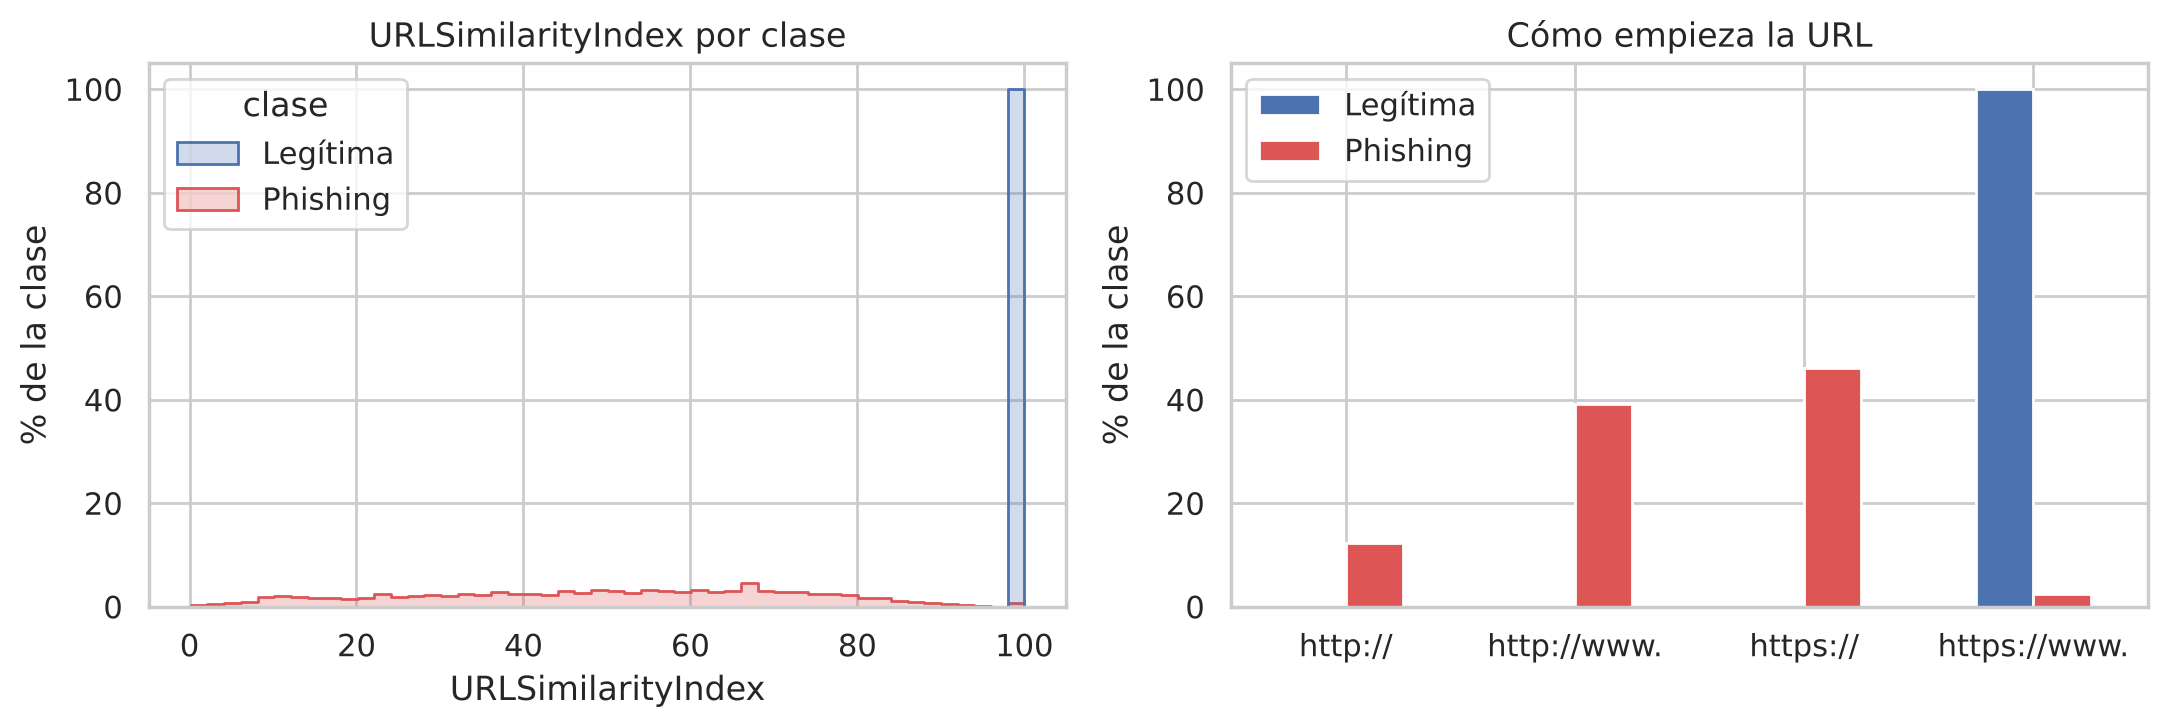
\includegraphics[width=\columnwidth]{03_atajos.png}
\caption{Distribución de \texttt{URLSimilarityIndex} y del prefijo de la URL por clase.}
\label{fig:atajos}
\end{figure}

\subsection{División de los datos}
Muchas URLs de phishing comparten dominio (por ejemplo, 1.192 URLs en \texttt{ipfs.io}). Para evitar que un modelo reconozca dominios ya vistos, la división en entrenamiento, validación y prueba (70/15/15~\%) se hizo agrupando por dominio: 164.918, 35.206 y 35.246 URLs, con cerca de 42~\% de phishing en cada conjunto. La validación se usó para comparar y ajustar modelos, y el conjunto de prueba se usó una sola vez al final.

\section{Metodología}

\subsection{Enfoque A: modelos tabulares}
Se compararon regresión logística, Random Forest (150 árboles), XGBoost~\cite{chen2016} y un perceptrón multicapa (capas de 64 y 32 neuronas). Para la regresión logística y el perceptrón, las variables se transformaron con $\log(1+x)$ y se estandarizaron. Se definieron cuatro escenarios, de más a menos atajos: A1, las 50 variables; A2, sin \texttt{URLSimilarityIndex}; A3, solo las 21 variables de la URL; y A4, 46 variables léxicas propias calculadas únicamente con el dominio (largo, puntos, guiones, dígitos, proporción de vocales, entropía de Shannon, palabras como \emph{login} o \emph{secure} y TLD). Los hiperparámetros de XGBoost en A4 se ajustaron con una grilla de 12 combinaciones de profundidad, tasa de aprendizaje y peso mínimo por hoja, con detención temprana en validación.

\subsection{Enfoque B: modelos de texto}
Los modelos de texto reciben tres entradas: la URL original, la URL normalizada (sin esquema, sin \texttt{www.} y sin la barra final) y solo el dominio. Se compararon: (i) TF-IDF de n-gramas de 2 a 4 caracteres (100.000 términos) con regresión logística; (ii) una CNN de caracteres con \emph{embedding} de 32 dimensiones, filtros convolucionales de anchos 2 a 5 (64 por ancho), \emph{global max pooling}, una capa densa de 64 neuronas y \emph{dropout} de 0,3; y (iii) una BiGRU de 32 unidades por dirección. Las redes se entrenaron en Keras con Adam (tasa $10^{-3}$), entropía cruzada binaria, lotes de 256 y detención temprana (paciencia 3, máximo 25 épocas). El dominio se truncó a 64 caracteres y la URL a 128.

\subsection{Evaluación}
La clase positiva es phishing. Se reportan precisión, \emph{recall}, F1 y ROC-AUC. Para cada escenario se seleccionó el modelo con mayor F1 en validación. Las predicciones de XGBoost se explicaron con SHAP~\cite{lundberg2017}.


\section{Resultados}

\subsection{Resultados en el conjunto de prueba}
La Tabla~\ref{tab:test} y la Fig.~\ref{fig:test} muestran el desempeño en prueba del modelo seleccionado en cada escenario. Todos los modelos que usan las variables originales o la URL completa obtienen F1 entre 0,996 y 1,000; el Random Forest con las 50 variables no comete errores en las 35.246 URLs. Quitar \texttt{URLSimilarityIndex} (A2) o las variables de la página (A3) no cambia este resultado, porque las variables de la URL se calcularon sobre la URL completa y también reflejan el prefijo y la ruta. En A1 y A2 incluso la regresión logística supera 0,999 en validación, otra señal de que el problema, tal como está planteado, es artificialmente fácil.

\begin{table}[t]
\caption{Resultados en prueba (clase positiva: phishing)}
\label{tab:test}
\centering
\setlength{\tabcolsep}{4pt}
\begin{tabular}{llcccc}
\toprule
Modelo & Entrada & P & R & F1 & AUC \\
\midrule
RF & A1: 50 variables & 1,000 & 1,000 & 1,000 & 1,000 \\
MLP & A2: 49 variables & 1,000 & 1,000 & 1,000 & 1,000 \\
MLP & A3: 21 de la URL & 1,000 & 0,995 & 0,997 & 0,999 \\
TF-IDF + RL & URL original & 1,000 & 0,993 & 0,996 & 0,999 \\
CNN & URL original & 1,000 & 0,995 & 0,997 & 0,999 \\
TF-IDF + RL & URL normalizada & 0,946 & 0,814 & 0,875 & 0,943 \\
\midrule
TF-IDF + RL & Dominio & 0,913 & 0,762 & \textbf{0,830} & 0,919 \\
CNN & Dominio & 0,952 & 0,728 & 0,825 & 0,919 \\
BiGRU & Dominio & 0,953 & 0,709 & 0,813 & 0,910 \\
XGBoost & A4: léxicas del dominio & 0,921 & 0,672 & 0,777 & 0,881 \\
\bottomrule
\multicolumn{6}{l}{\footnotesize Sobre la línea: usan atajos. Bajo la línea: solo el dominio.}
\end{tabular}
\end{table}

\begin{figure}[t]
\centering
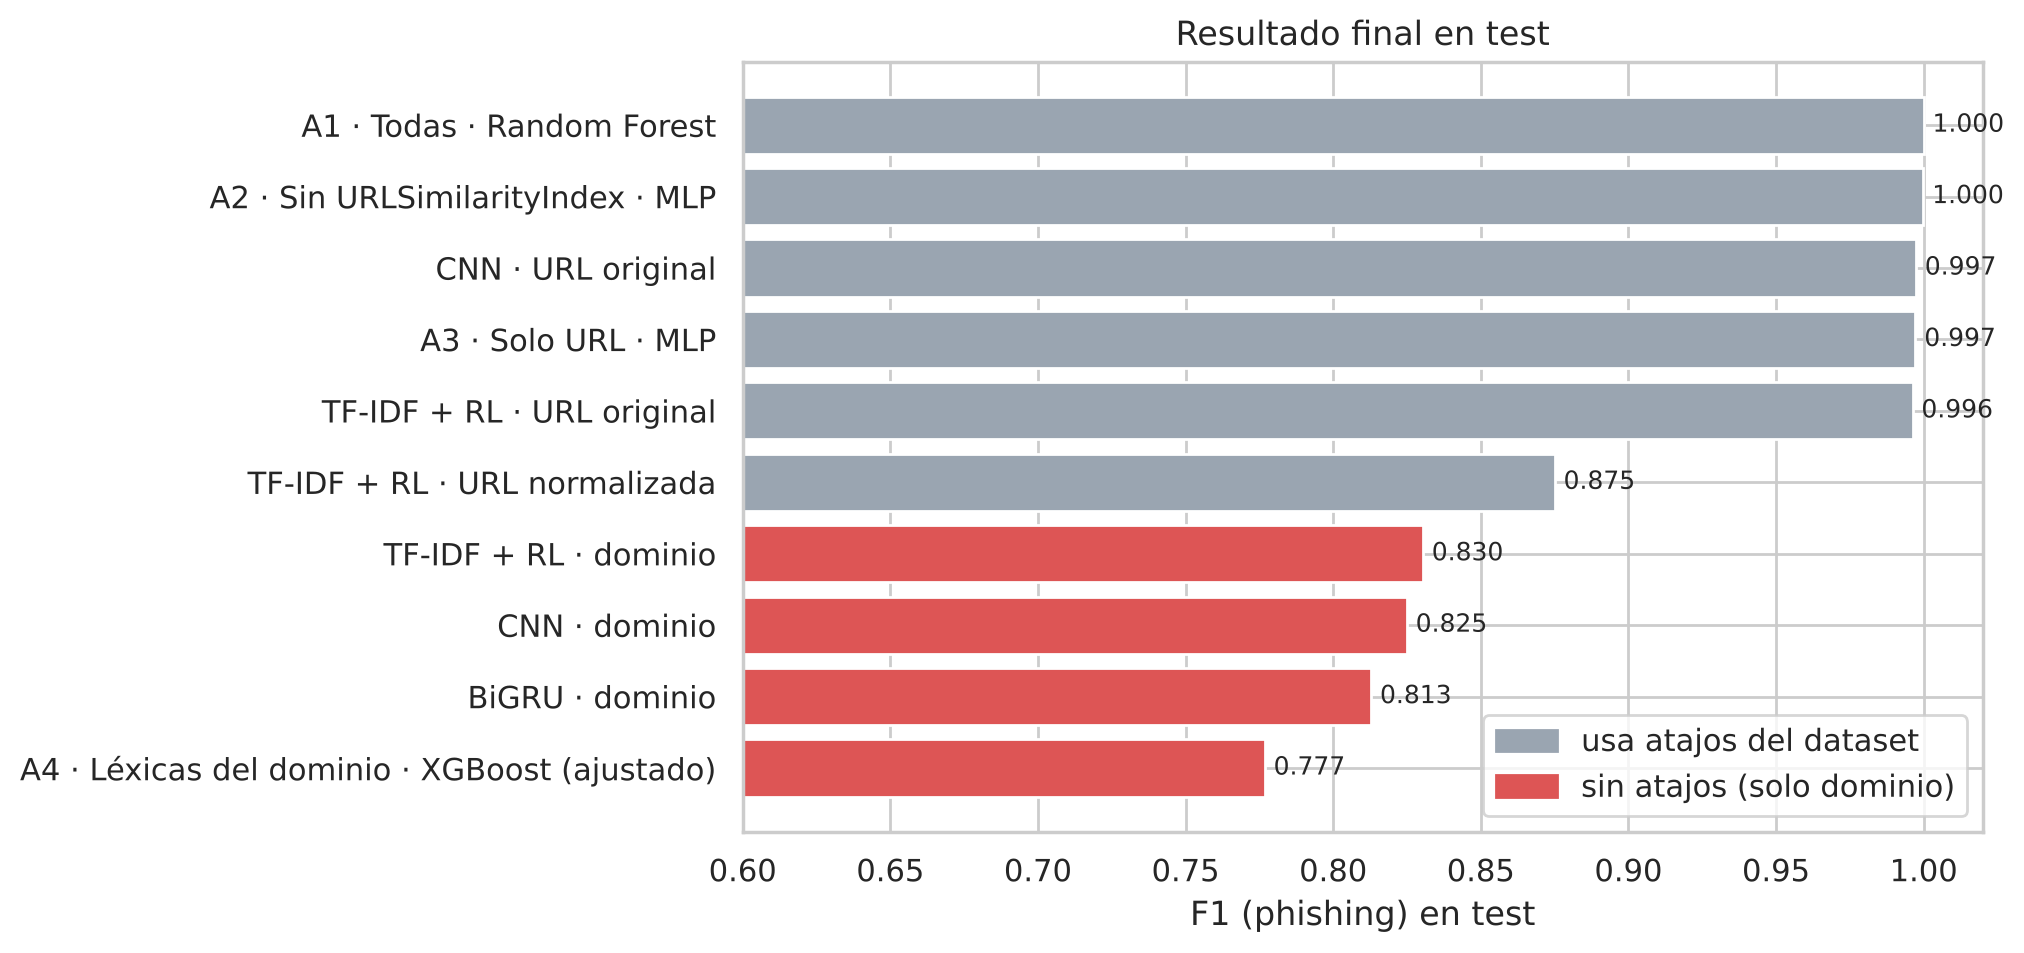
\includegraphics[width=\columnwidth]{12_resultados_test.png}
\caption{F1 en prueba. En gris, los modelos que usan atajos; en rojo, los que solo ven el dominio.}
\label{fig:test}
\end{figure}

Sin atajos, el desempeño cae a F1 $\approx$ 0,83. Entre los modelos de dominio, TF-IDF con regresión logística (0,830) y la CNN de caracteres (0,825) quedan prácticamente empatados, con el mismo ROC-AUC (0,919); la CNN es más precisa (0,952 frente a 0,913) y TF-IDF detecta más phishing (\emph{recall} 0,762 frente a 0,728). La BiGRU queda algo por debajo (0,813) y tarda más del doble en entrenarse en CPU. Los tres modelos de texto superan en 4 a 5 puntos de F1 al mejor modelo con variables léxicas hechas a mano (XGBoost, 0,777), cuyo ajuste de hiperparámetros aportó cerca de un punto de F1 en validación. Con textos cortos como un dominio, los n-gramas de caracteres ya capturan gran parte de la información disponible, por lo que la red neuronal no supera con claridad a una línea base bien construida.

\begin{figure*}[t]
\centering
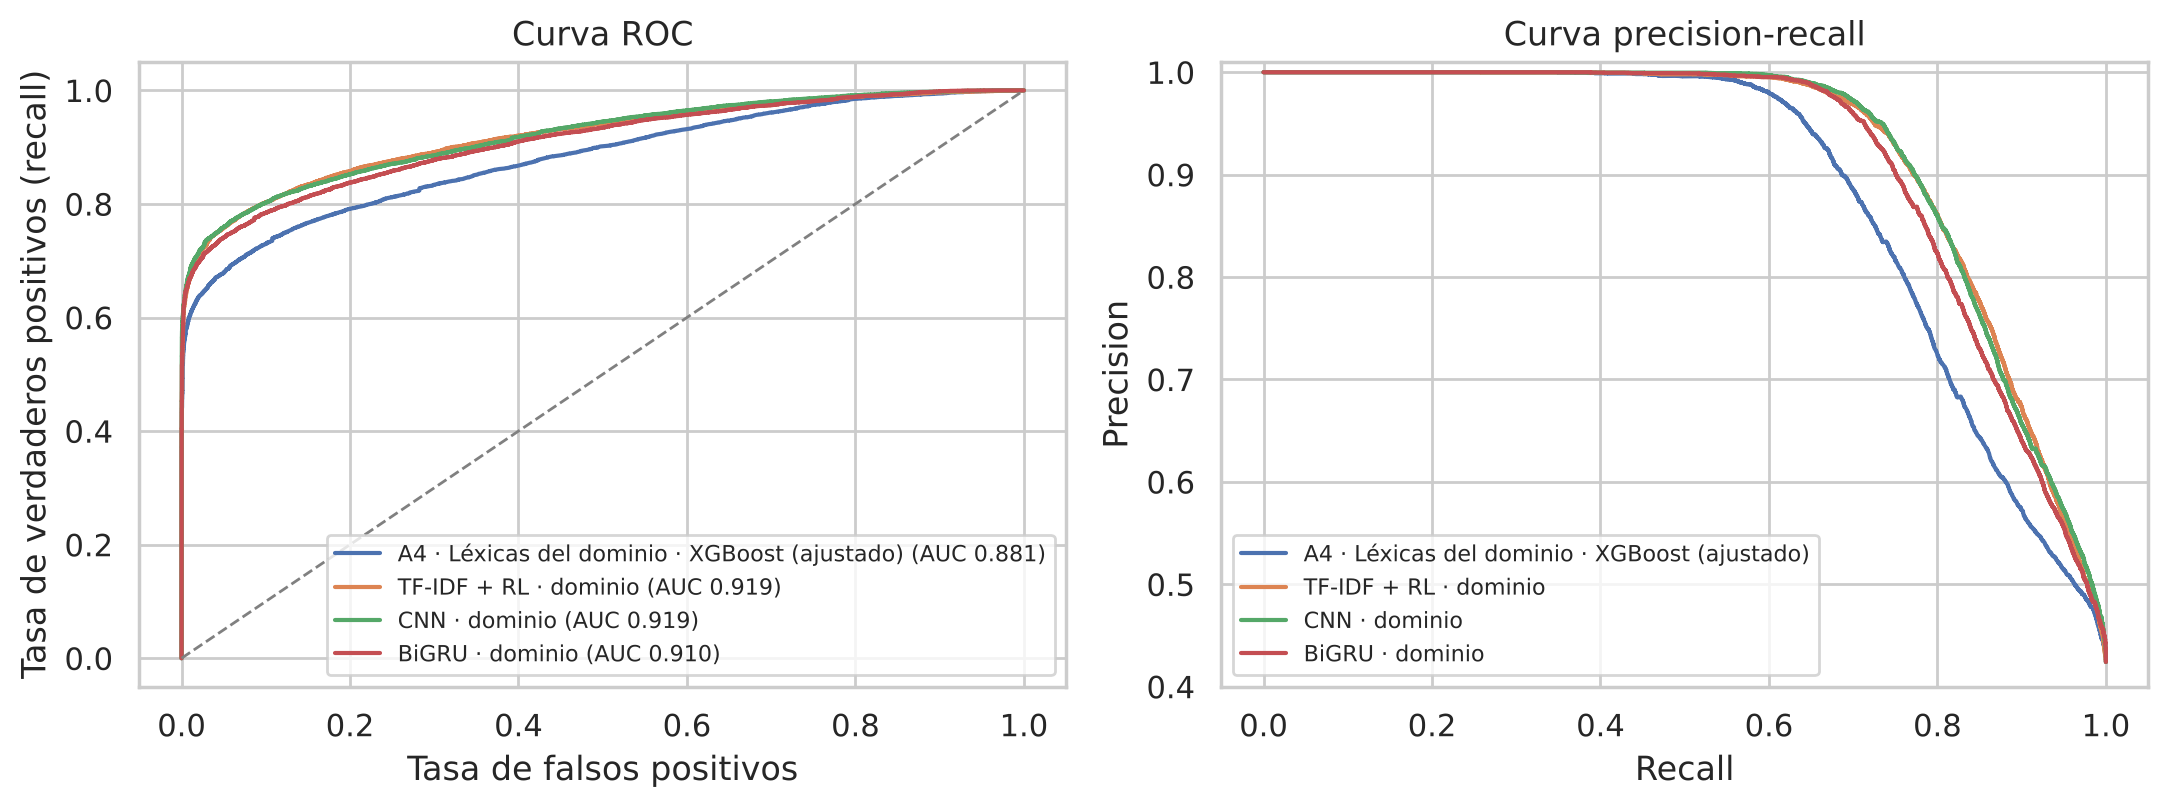
\includegraphics[width=0.8\textwidth]{14_roc_pr_dominio.png}
\caption{Curvas ROC y precisión-\emph{recall} en prueba de los modelos que solo ven el dominio.}
\label{fig:roc}
\end{figure*}

La Fig.~\ref{fig:roc} muestra que las curvas de TF-IDF y de la CNN prácticamente se superponen, y que ambas dominan a XGBoost con variables léxicas en todo el rango de umbrales.

\subsection{Interpretación}
Con SHAP, el modelo de A2 se apoya sobre todo en variables de la página (líneas de código, referencias propias y externas) y en \texttt{IsHTTPS}, que reflejan el modo de recolección. En A4, las variables más influyentes son la cantidad de puntos del dominio, su largo, los dígitos y el largo del TLD. Los n-gramas con mayor peso hacia phishing en el modelo TF-IDF corresponden a TLDs gratuitos o de bajo costo (\texttt{.cf}, \texttt{.ga}, \texttt{.ml}, \texttt{.top}); hacia legítima, a \texttt{.gov}, \texttt{.edu}, \texttt{.mil} y TLDs de países.

\subsection{Prueba con URLs fuera del dataset}
Para comprobar el efecto de los atajos se clasificaron URLs escritas a mano (Tabla~\ref{tab:manual}). La CNN entrenada con la URL original asigna probabilidad 1,000 de phishing a cinco URLs legítimas reales, solo porque tienen ruta o subdominio. La CNN de dominio clasifica bien \texttt{github.com}, pero deja \texttt{google.com} y \texttt{es.wikipedia.org} cerca del umbral y marca \texttt{mail.google.com} como phishing.

\begin{table}[t]
\caption{Probabilidad de phishing en URLs escritas a mano}
\label{tab:manual}
\centering
\resizebox{\columnwidth}{!}{%
\begin{tabular}{lcc}
\toprule
URL & CNN URL & CNN dominio \\
\midrule
\multicolumn{3}{l}{\emph{Legítimas}} \\
\texttt{https://www.google.com/maps} & 1,000 & 0,527 \\
\texttt{https://es.wikipedia.org/wiki/Phishing} & 1,000 & 0,592 \\
\texttt{https://github.com/54isaac09} & 1,000 & 0,320 \\
\texttt{https://www.ubiobio.cl/w/} & 1,000 & 0,604 \\
\texttt{https://mail.google.com/mail/u/0/} & 1,000 & 0,998 \\
\multicolumn{3}{l}{\emph{Phishing inventadas}} \\
\texttt{http://secure-login-verify-account.xyz/signin} & 1,000 & 1,000 \\
\texttt{http://192.168.10.5/bank/login.php} & 1,000 & 1,000 \\
\bottomrule
\end{tabular}}
\end{table}

Esto revela un sesgo residual en el dominio: solo el 4~\% de los dominios legítimos tiene subdominio (además de \texttt{www}), frente al 55~\% de los de phishing, y hay 921 URLs de phishing con ``google'' en el dominio (por ejemplo, formularios en \texttt{docs.google.com}) frente a 12 legítimas. Por lo tanto, el F1 de 0,83 también es optimista respecto de un escenario real.

\subsection{Umbral y errores}
Con el umbral por defecto (0,5) la CNN de dominio deja pasar 4.068 URLs de phishing. Un umbral de 0,16, elegido en validación para alcanzar 90~\% de \emph{recall}, logra 0,894 de \emph{recall} en prueba, pero la precisión baja a 0,669. Los phishing no detectados se parecen a dominios comunes: el 40,9~\% de los que terminan en \texttt{.com} se escapa, frente al 17,2~\% del resto, y solo el 3,9~\% de los que contienen dígitos.

\section{Conclusiones}

Se implementó y evaluó una rutina completa de detección de URLs de phishing con siete modelos de Machine Learning y Deep Learning sobre PhiUSIIL. Con las variables originales o la URL completa, todos los modelos alcanzan F1 entre 0,996 y 1,000, en línea con lo reportado para este dataset. Sin embargo, el análisis exploratorio mostró que este desempeño se explica por tres atajos: las URLs legítimas siempre comienzan con \texttt{https://www.}, nunca tienen ruta y siempre tienen \texttt{URLSimilarityIndex} = 100. Un modelo entrenado con la URL original clasifica como phishing cualquier URL legítima con ruta, por lo que su exactitud no se trasladaría a un uso real.

Al eliminar los atajos y usar solo el dominio, el mejor F1 en prueba fue 0,830 (TF-IDF con regresión logística), seguido de cerca por la CNN de caracteres (0,825), que fue la más precisa. Los modelos que aprenden de los caracteres superan a las variables léxicas diseñadas a mano.

Las principales limitaciones son el uso de un solo dataset, el sesgo residual de los dominios legítimos (sin subdominios) y la imposibilidad de distinguir, solo con el dominio, el phishing alojado en servicios legítimos. Como trabajo futuro se propone evaluar los modelos con otra fuente de URLs, construir un conjunto con URLs legítimas que incluyan rutas y subdominios, combinar dominio y ruta en ese conjunto y explicar las predicciones de la CNN.


\bibliographystyle{IEEEtran}
\bibliography{referencias}

\end{document}
